%-------------------------------------------------------------------------------
%-------------------------------------------------------------------------------
\section{Processus de branchement} \label{sec:Proba-Branchement}
%-------------------------------------------------------------------------------

%-------------------------------------------------------------------------------
\paragraph*{Processus de (Bienaymé-)Galton-Watson.}
On suit une population au cours des générations. A chaque génération, chaque individu peut avoir des descendants, qui peuvent avoir eux-même des descendants, etc. On constitue ainsi un processus de branchement qui reflète la généalogie des individus.

Si on part d'un seul individu, et qu'on note $X_{0, 1}$ le nombre de ses descendants, et $X_{1, 1}$, $X_{1, 2}$, \dots le nombre de descendants de chacun de ces descendants, on voit que la taille de la population vaut successivement
\begin{align*}
  Z_1 & = X_{0, 1}, &
  Z_2 & = \sum_{i=1}^{Z_1} X_{1, i}, &
  Z_3 & = \sum_{i=1}^{Z_2} X_{2, i}, &
  \dots
\end{align*}

%-------------------------------------------------------------------------------
\subsection{Fonction génératrice des probabilités} 
%-------------------------------------------------------------------------------

Les fonctions génératrices (il en existe plusieurs) permettent de manupuler facilement des combinaisons (notamment des sommes) de variables aléatoires.

\begin{definition}[Fonction génératrice]
  Soit $X$ une variable aléatoire positive. On note $f_X$ sa {\em fonction génératrice des probabilités} (= '{\em pgf}') définie comme
  $$
  \begin{array}{rrcl}
    f_X : & [0, 1] & \mapsto & [0, 1] \\
      & s & \to & f_X(s) = \Esp\left(s^X\right).
  \end{array}
  $$
\end{definition}

\remark
On voit facilement que $f_X(1) = 1$ et que $f_X$ est monotone croissante.

%-------------------------------------------------------------------------------
\paragraph*{Fonction génératrices de quelques lois de probabilités.}
\begin{description}
  \item[Bernoulli:] si $X \sim \Bcal(p)$ 
  $$
  f_X(s) = (1-p) s^0 + p s^1 = 1 - p + p s.
  $$
  Notamment, si $p = 1$, $f_X(s) = s$.
  \item[Binomiale:] si $X \sim \Bcal(n, p)$
  $$
  f_X(s) = \sum_{k=0}^n {{n}\choose{k}} (1-p)^{n-k} (ps)^k = (1 - p + ps)^n.
  $$
  \item[Géométrique:] si $X \sim \Gcal(a)$ ($\Pr\{X = k\} = (1-a) a^k$ pour $k \geq 0$)
  $$
  f_X(s) = (1-a) \sum_{k=0}^n (as)^k = \frac{1-a}{1 - as}.
  $$
  \item[Poisson:] si $X \sim \Pcal(\lambda)$
  $$
  f_X(s) = e^{-\lambda} \sum_{k\geq0} (\lambda s)^k / (k!) = e^{-\lambda} e^{\lambda s} = \exp(\lambda(s-1)).
  $$
\end{description}

%-------------------------------------------------------------------------------
\paragraph*{Quelques propriétés des fonctions génératrices de probabilités.}

\begin{proposition}
  La fonction génératrice $f_X$ est $C^\infty$ sur $[0, 1]$ et sa $k$-ème dérivée vaut
  \begin{align*}
    f_X^{(k)}(s) 
    & = \sum_{n \geq k} \Pr\{X = n\} n(n-1)  \dots (n-k+1) s^{X-k} \\
    & = \Esp(X (X-1) \dots (X-k+1) s^{X-k})
  \end{align*}
\end{proposition}

\proof
  $C^\infty$ non démontré. Formule de $f_X^{(k)}(s)$ directe comme dérivées successives de $s^n$.
\eproof

\begin{corollary}
  En conséquence, on a
  \begin{align*}
    \forall k \geq 0: \quad \Pr\{X = k\} & = f_X^{(k)}(0) / (k!), \\
    \Esp(X) & = f'_X(1), &
    \Esp(X(X-1)) & = f''_X(1).
  \end{align*}
\end{corollary}

\proof 
Directe.
\eproof.

\remarks
\begin{enumerate}
  \item Le corollaire justifie le nom de 'fonction génératrice des probabilités'. $F_X$ nous donne également les moments de $X$. Notamment
  \begin{align*}
    \Var(X) 
    & = \Esp(X^2) - (\Esp X)^2 \\
    & = \Esp(X(X-1) + X) - (\Esp X)^2
    = \Esp(X(X-1)) + \Esp X - (\Esp X)^2 \\
    & = f''_X(1) + f'_X(1)(1 - f'_X(1)). 
  \end{align*}
  \item En fait, la fonction génératrice caractérise complètement la loi de la variable $X$. Elle permet également d'assurer la convergence en loi.
\end{enumerate}

%-------------------------------------------------------------------------------
% \progres{
% Rappel cours 8 :
% \begin{itemize}
%   \item Fin chaînes de Markov, processus de Wright-Fisher, marche aléatoire
%   \item Processus de branchement
%   \item Fonction génératrice
% \end{itemize}
% Programme cours 9 :
% \begin{itemize}
%   \item Processus de Galton-Watson
%   \item TD chaînes de Makov, processus de branchement
% \end{itemize}
% }

%-------------------------------------------------------------------------------
\begin{proposition}[Convergence de la fonction génératrice]
  Soient $(X_n)_{n \geq 0}$ une suite de variables aléatoires positives et $X$ un variable aléatoires positives :
  $$
  (X_n)_{n \geq 0} \overset{\Lcal}{\longrightarrow} X
  \qquad \Leftrightarrow \qquad
  \forall s \in [0, 1]: \quad \lim_{n \to \infty} f_{X_n}(s) = f_X(s).
  $$
\end{proposition}

\proof Non démontrée. \eproof

\begin{proposition}[Fonction génératrice de la somme]
  Soient $X$ et $Y$ deux variables aléatoires positives indépendantes, on a
  $$
  f_{X+Y}(s) = f_X(s) \; f_Y(s).
  $$
\end{proposition}

\proof
Il suffit de partir de la définition et d'utiliser l'indépendance :
$$
f_{X+Y}(s) 
= \Esp(s^{X+Y}) = \Esp(s^X \; s^Y) = \Esp(s^X) \;  \Esp(s^Y)
= f_X(s) \; f_Y(s).
$$
\eproof

\remarks
\begin{enumerate}
  \item Une conséquence directe est que si $X_1$, $X_2$, \dots $X_n$ sont positives et iid, alors la fonction génératrice de leur somme vaut
  $$
  f_{X_1 + \dots + X_n}(s) = \left(f(X_1)\right)^n.
  $$
  \item Cette propriété donne une autre démonstration de la formule de $f_X$ pour la loi binomiale, vue comme une somme de $n$ variables de Bernoulli indépendantes.
\end{enumerate}

\begin{proposition}[Fonction génératrice d'une somme en nombre aléatoire] \label{prop:fGeneratriceSommeAleatoire}
  Soient $(X_n)_{n \geq 1}$ une suite de variables aléatoires positives iid et $N$ une variables positive indépendante, on s'intéresse à la somme des $N$ premiers éléments de la suite :
  $$
  Z = \sum_{n=1}^N X_n.
  $$
  On a 
  $$
  f_{Z}(s) = f_N \circ f_X(s).
  $$
\end{proposition}

\proof
On conditionne par $N$ :
\begin{align*}
  f_Z(s) 
  = \Esp_N \left(\Esp(e^Z \mid N) \right)
  = \Esp_N \left(f_X(s)^N \right)
  = f_N \left(f_X(s)^N \right) = f_N \circ f_X(s).
\end{align*}

\eproof

%-------------------------------------------------------------------------------
\subsection{Processus de Galton-Watson (GW)} 
%-------------------------------------------------------------------------------

On reprend une population évoluant de la façon décrite au début de la section. 
On note $Z_n$ la taille de la population à la $n$-ème génération ($n \geq 0$) et $X_{ni}$ le nombre de descendants du $i$ individu de la $n$-ème génération. 
On suppose que les $\{X_{ni})_{n \geq 0, 1 \geq i \geq Z_n}$ sont iid (et indépendants de $Z_0$).

\bigskip
La taille de la population à la génération $n+1$ est donnée par 
\begin{equation} \label{eq:recurrenceGW}
Z_{n+1} = \sum_{i = 1}^{Z_n} X_{ni}.
\end{equation}

La suite $(Z_n)_{n \geq 0}$ forme donc une \cM sur $\Nbb$, puisque $Z_{n+1}$ est donné par $Z_n$ et par les $\{X_{ni})_{1 \geq i \geq Z_n}$, qui sont indépendants du passé.

\bigskip
On s'intéresse notamment à l'événement d'extinction défini par 
$$
Ext = \{T_0 < \infty\}.
$$
et à la probabilité d'extinction partant d'une population de taille 1 : 
$$
q := \Pr_1\{Ext\}.
$$


%-------------------------------------------------------------------------------
\paragraph*{Matrice de transition.} 
On peut caractériser les probabilités de transition 
$$
p_{ij} = \Pr\{Z_{n+1} = j \mid Z_n = i\}
$$
par leur fonction génératrice. En effet, \eqref{eq:recurrenceGW} donne
$$
\Esp(s^{Z_{n+1}} \mid Z_n) = f_X^{Z_n}(s)
\qquad \Rightarrow \qquad 
\sum_{j \geq 0} p_{ij} s^j = \Esp(s^{Z_{n+1}} \mid Z_n=i) = f_X(s)^i,
$$
donc
$$
p_{ij} = \frac{\left(f_X(0)^i\right)^{(j)}}{j!}.
$$
On observe qu'il s'agit bien d'une \cM homogène (puisque la fonction génératrice ne dépend par de $n$).

%-------------------------------------------------------------------------------
\paragraph*{Classification des états.} 
\begin{itemize}
 \item L'état $\{0\}$ ne communique avec aucun autre : il constitue donc une classe à lui seul. Comme il est de plus impossible d'en sortir ($p_{00} = 1$), il est récurrent : on parle d'état absorbant.
 \item Si $\Pr\{X \geq 2\} > 0$, tous les autres états communiquent, ils constituent donc une unique classe et possède tous la même nature.
 \item On peut montrer que tous les états, hormis $\{0\}$ sont transients.
\end{itemize}

Le caractère transient des états non nuls signifie qu'ils ne sont visités qu'un nombre fini de fois, ce qui signifie que soit la \cM est absorbée en 0, soit elle part vers l'infini : 
$$
\Pr_\mu\left\{ \lim_{n \to \infty} Z_n = + \infty\right\} = 1 - \Pr_\mu\{Ext\}.
$$

%-------------------------------------------------------------------------------
\paragraph*{Extinction de la population.} 
On suppose que $f_X(0) \notin \{0, 1\}$, c'est-à-dire que 
$$
0 < \Pr\{X = 0\} < 1.
$$

\remark
$\Pr\{X = 0\} = 1$ implique une extinction immédiate de la population et $\Pr\{X = 0\} = 0$, au contraire, interdit l'extinction.

\begin{proposition}
  La probabilité d'extinction $q$ est un point fixe de la fonction génératrice de $X$ :
  $$
  q = f_X(q).
  $$
\end{proposition}

\proof
On commence par remarquer que la probabilité d'extinction partant de $k$ individus indépendants vaut
$$
\Pr_k\{Ext\} = \left(\Pr_1\{Ext\}\right)^k = q^k,
$$
puisqu'il faut pour cela que les $k$ populations indépendantes s'éteignent. En sommant sur toutes les tailles possibles à la première génération on a donc
$$
q 
= \Pr_1\{Ext\} 
= \sum_{k \geq 0} \Pr_1\{Z_1 = k\} \Pr_k\{Ext\}
= \sum_{k \geq 0} \Pr_1\{Z_1 = k\} q^k
= f_{Z_1}(q)
= f_X(q).
$$

\begin{proposition} \label{prop:fonctionGeneratriceZn}
  La fonction génératrice de $Z_n$ partant de $Z_0 = 1$ est
  $$
  f_{Z_n}(s) = \Esp_1(s^{Z_n}) = \underset{n \text{ fois}}{\underbrace{f_X \circ f_X \circ \dots \circ f_X}}(s).
  $$
\end{proposition}

\proof 
C'est une conséquence directe de la proposition \ref{prop:fGeneratriceSommeAleatoire} : puisque
$$
Z_n = \sum_{i=1}^{Z_{n-1}} X_{n-1, i},
$$
on a la récurrence 
\begin{equation} \label{eq:recurrenceFonctionGeneratriceGW}
f_{Z_n} = f_{Z_{n-1}} \circ f_X
\end{equation}
et la preuve se conclue en remarquant que $f_{Z_1} = f_X$, puisque $Z_0 = 1$.
\eproof

\begin{definition}
  Soit $m = \Esp(X) = f'_X(1)$ le nombre moyen de descendants. Le processus GW est dit critique si $m=1$, sous-critique si $m < 1$ et sur-critique si $m > 1$.
\end{definition}

\remarks
\begin{enumerate}
  \item La récurrence \eqref{eq:recurrenceFonctionGeneratriceGW} nous assure notamment que
  $$
  \Esp(Z_n) = m \Esp(Z_{n-1}),
  $$
  en effet
  \begin{align*}
    \Esp(Z_n) 
    = f'_{Z_n}(1) = (f_{Z_{n-1}} \circ f_X)'(1) 
    = f'_X(1) \times f'_{Z_{n-1}}\left(f_X(1)\right) 
    = m f'_{Z_{n-1}}(1) = m \Esp(Z_{n-1}).
  \end{align*}
  Notamment, partant de $Z_0 = 1$, on a $\Esp_1(Z_n) = m^n$.
  \item Dans le cas où $Z_0$ est aléatoire, de fonction génératrice $f_{Z_0}$, on obtient de la même manière
  $$
  f_{Z_n} =  f_{Z_0} \circ \underset{n \text{ fois}}{\underbrace{f_X \circ f_X \circ \dots \circ f_X}}.
  $$
\end{enumerate}

\begin{lemma} \label{lem:GWnombrePointsFixes}
  Si $f_X(0) > 0$, $f_X$ admet pour points fixes dans $[0, 1]$
  \begin{align*}
    \{s = 1\} & \text{ si } m \leq 1, &
    \{0 < s_1 < 1, s_2=1\} & \text{ si } m > 1.
  \end{align*}
\end{lemma}

\proof
Nous allons montrer que la position du nombre moyen de descendants $m$ par rapport à 1 contrôle le nombre de points fixes de $f_X$.
Pour cela, on distingue les deux cas $\Pr\{X\geq 2\} = 0$ ou $\Pr\{X\geq 2\} > 0$.
\begin{itemize}
  \item Si $\Pr\{X\geq 2\} = 0$, alors $X \in \{0, 1\}$, donc c'est une variable de Bernoulli $\Bcal(m)$ et $f_X(s)$ est linéaire, de pente $m \leq 1$. $f_X$ ne croise donc la première bissectrice qu'en $s = 1$.
  \item Si $\Pr\{X\geq 2\} > 0$, alors
  \begin{align*}
  f'_X(s) 
  & = \Esp(X s^{X-1}) 
  = s^{-1} \Esp(X s^X) > 0 
  & & \text{pour} \quad s > 0, 
  \\
  f''_X(s) 
  & = \Esp(X(X-1) s^{X-2}) \\
  & = \sum_{x \geq 2} x (x-1) s^x 
  = \sum_{x \geq 0} (x+2) (x+1) s^x 
  > 0 
  & & \text{pour} \quad 0 < s \leq 1.
  \end{align*}
  La fonction $f_X$ est donc monotone croissante sur $(0, 1]$ et strictement convexe sur $(0, 1]$ avec $f_X(0) = \Pr\{X = 0\} > 0$. Son graphe coupe donc la première bissectrice 
  \begin{itemize}
  \item en $s^* < 1$ et en 1 si $f'_X(1) = m > 1$,
  \item en 1 seulement si $f'_X(1) = m \leq 1$.
  \end{itemize}
\end{itemize}
\eproof

$$
\begin{tabular}{cc}
  \begin{tabular}{l}
    \textcolor{red}{\bf --} : $m < 1$ \\ ~ \\
    \textcolor{green}{\bf --} : $m = 1$ \\ ~ \\
    \textcolor{blue}{\bf --} : $m > 1$
  \end{tabular}
  &
  \begin{tabular}{c}
  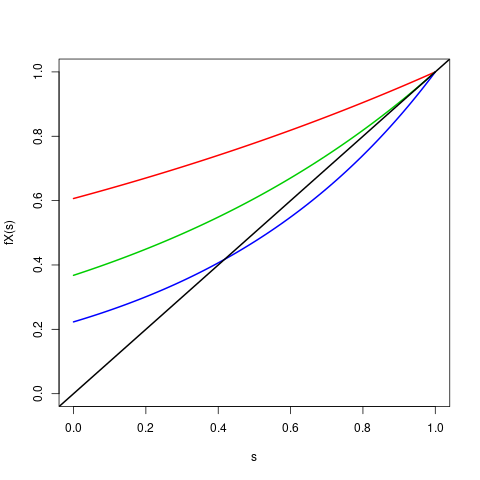
\includegraphics[width=.4\textwidth]{GaltonWatson-pgf}
  \end{tabular}
\end{tabular}
$$

\remarks
\begin{enumerate}
  \item On voit ainsi que la probabilité d'extinction vaut $q = 1$ si le processus est sous-critique ($m < 1$) ou critique ($m = 1$, puisque $\Pr\{X = 0\} > 0$). 
  \item Il reste à étudier le cas sur-critique pour déterminer quel point fixe donne la probabilité d'extinction.
\end{enumerate}

\begin{proposition}
  La probabilité d'extinction $q$ est la plus petite solution de l'équation de point fixe $s = f_X(s)$.
\end{proposition}

\proof
On note, pour $n \geq 1$, la probabilité que la population soit éteinte à la génération $n$ :
$$
q_n := f_{Z_n}(0) = \Pr_1\{Z_n = 0\} = \Pr_1\{T_0 \leq n\}.
$$
Par définition de $q$, on a
$$
q = \lim_{n \to \infty} q_n.
$$
Par la proposition \ref{prop:fonctionGeneratriceZn} on a:
$$
q_{n+1} = f_{Z_{n+1}}(0) = f_X \circ f_{Z_n} (0) = f_X(\Pr_1\{Z_n = 0\}) = f_X(q_n).
$$
(On retrouve que la limite $q$ de la suite $(q_n)_{n \geq n}$ doit vérifier $q = f_X(q)$.) \\
% $q$ est donc bien un point fixe de $f$. Le lemme \ref{lem:GWnombrePointsFixes} indique que leur nombre dépend de la position de $m$ par rapport à 1. Il reste montrer que $q$ est le plus petit d'entre eux, noté $s^*$. \\
% % La convergence vers le plus petit point fixe s'obtient en remarquant que, puisque $Z_0 = 1$, on a $q_0 = 0$ et en considérant la figure ci-dessous qui s'appuie sur le fait que $f_X(s) > s$ pour $s$ inférieur au plus petit point fixe.
% On note, pour $n \geq 0$:
% $$
% q_n := \Pr_1\{Z_n = 0\}.
% $$
% Par la proposition \ref{prop:fonctionGeneratriceZn}, on a:
% $$
% q_{n+1} = f_{Z_{n+1}}(0) = f_X \circ f_{Z_n} (0) = f_X(\Pr_1\{Z_n = 0\}) = f_X(q_n).
% $$
La convergence de la suite $(q_n)_{n \geq 0}$ vers le plus petit point fixe s'obtient en remarquant que $f_X$ est une fonction croissante et que, puisqu'elle est convexe sur $(0, 1]$, on a
$$
s < s^* \; \Rightarrow \; f_X(s) > s, \qquad \qquad
s > s^* \; \Rightarrow \; f_X(s) < s.
$$
$(q_n)_{n \geq 0}$ est donc une suite croissante si $q_0  < s^*$ et décroissante dans le cas contraire :
$$
\begin{tabular}{ccc}
  & $q_1 = .05$ & $q_1 = .75$ \\
  \begin{tabular}{lc}
    \textcolor{blue}{\bf --} : $f_X(s)$ \\ ~ \\
    \textcolor{red}{\bf --} : $(q_n)_{n \geq 0}$
  \end{tabular}
  &
  \begin{tabular}{cc}
  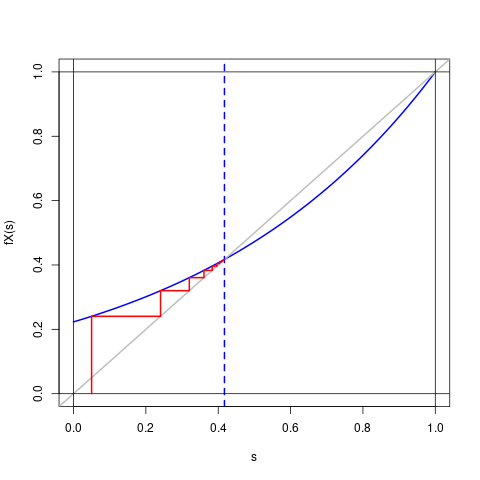
\includegraphics[width=.4\textwidth, trim=0 10 25 50, clip=]{GaltonWatson-fixPoint-q05}
  \end{tabular}
  &
  \begin{tabular}{cc}
  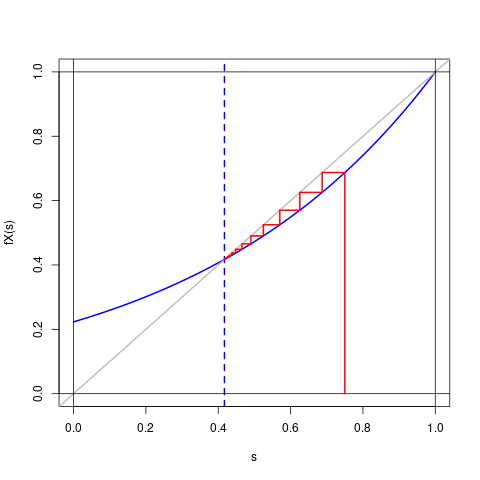
\includegraphics[width=.4\textwidth, trim=0 10 25 50, clip=]{GaltonWatson-fixPoint-q075}
  \end{tabular}
\end{tabular}
$$
\eproof

\remarks
\begin{enumerate}
  \item\todo{$q_n$ est croissante par construction, la trajectoire partant de $q_0 > s^*$ est donc impossible.}
  \item La convergence est donc démontrée pour $Z_0$ aléatoire, avec $q_0 = \Pr\{Z_0 = 0\} \in [0, 1)$ quelconque. Le cas $Z_0 = 1$ correspond au cas $q_0 = 0$.
  \item La convergence vers le point fixe $s^*$ peut également s'obtenir en montrant qu'il est contractant, c'est-à-dire que $|f'_X(s^*)| < 1$. Pour cela, on rapelle d'abord que $0 < f'_X(0) < 1$ et que $m = f'_x(1) > 1$. En appliquant le théorème des valeurs intermédiaire à $f'_X$, on conclue qu'il existe $\widetilde{s} \in (s^*, 1)$ tel que $f'_X(\widetilde{s}) = 1$. Comme enfin $f_X$ est strictement convexe, $f'_X(s)$ est strictement monotone croissante et donc $0 < f'_X(0) < f'_X(s^*) < f'_X(\widetilde{s}) = 1$.
\end{enumerate}


